\hypertarget{part-1-design-4}{
\section{Part 1, design 4}\label{part-1-design-4}}

\begin{figure}[ht]
  \centering
  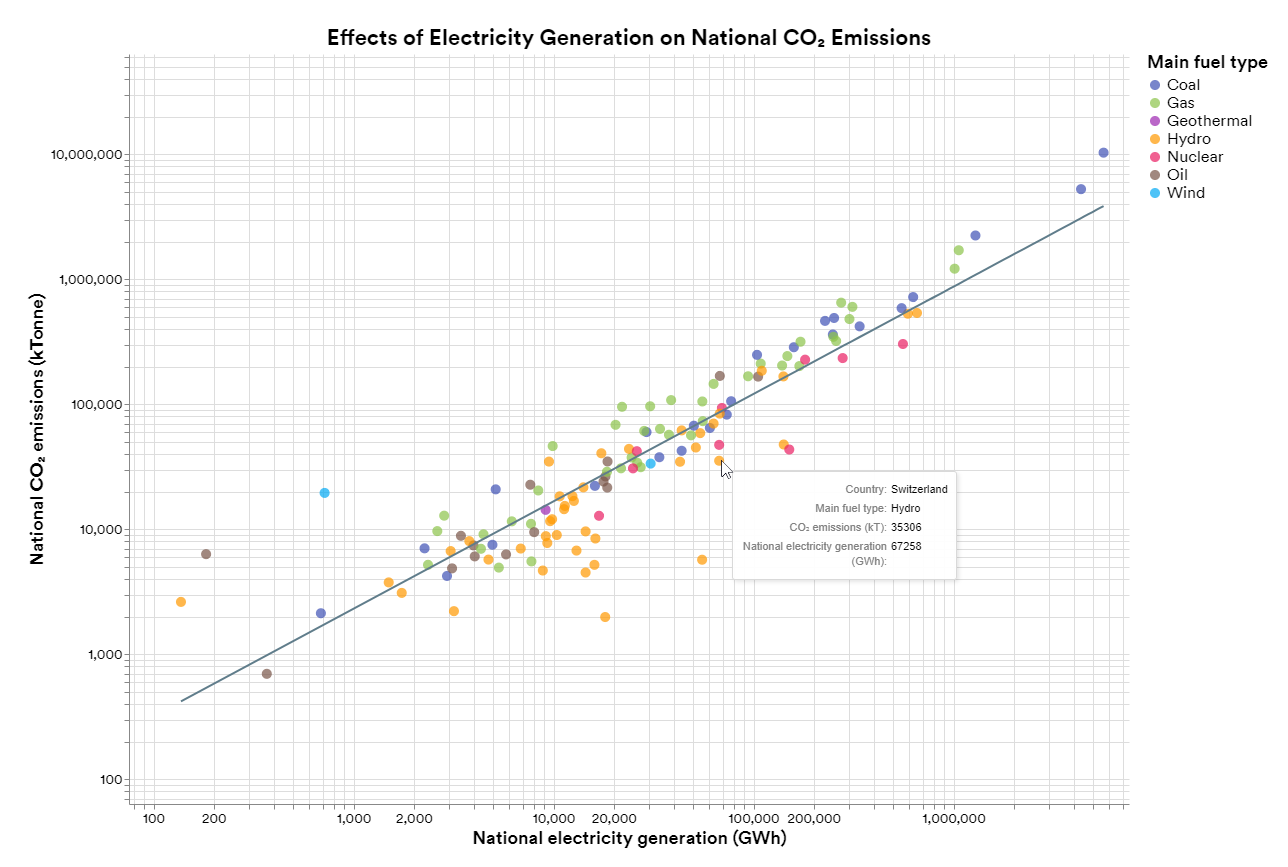
\includegraphics[width=\textwidth]{../img/design4}
  \caption{Effects of electricity generation on national CO$_2$ emissions (Design 4)}
\end{figure}

\hypertarget{description}{
\subsubsection{Description}\label{description}}

\begin{description}
\item[Visual Design Type:]
Interactive scatter plot
\item[Name of Tool:]
Altair
\item[Country:]
Worldwide
\item[Year:]
2014

\item[Visual Mappings:]
% each of the visual design mappings; include the data apping information about colour, shape, size, position (x/y axes), and any other visual mappings 
\begin{itemize}
  \item \textbf{Position}: Countries are represented as points on the chart, where their national power generation is compared with their national CO$_2$ emissions.
  \item \textbf{Hue}: The main fuel type of each country is indicated by the hue of the chart point.
  \item \textbf{Tooltips}: Tooltips are used to offer detail-on-demand to the user, showing exact generation and emissions figures.
  \item \textbf{Line of regression}: A computed line of regression is drawn over the points in order to evaluate countries' performance relative to the average.
  \item \textbf{Scroll}: An interactive chart means the user can drag and zoom the chart, allowing for points to be inspected with greater granularity.
\end{itemize}

\item[Unique Observation:]
% things we can learn from the visualisation e.g. from this vis we can see this pattern
The chart shows a strong correlation between national electricity generation and CO$_2$ emissions, and since the scale of the chart is logarithmic we can deduce that increased electricity generation correlates with an exponential increase in CO$_2$ emissions on a national level.

It is easy to compare countries in both generation and emissions, and the line of regression gives the user a baseline average from which countries' performance can be evaluated. For example, we can see that Switzerland with hydro power generates a similar amount of power to Finland with nuclear power, however Switzerland produces around 10,000 fewer kilotonnes of CO$_2$.

Additionally, more sweeping observations can be found, such as the trend for countries with gas as their main fuel tend to have above average CO$_2$ emissions as the green points largely appear above the trend line. Inversely, hydro power countries with yellow points tend to have less than average emissions.

\item[Data Preparation:]
% any modifications to the original data that had to be performed to generate your beautiful image
The provided GPPD data set was combined with a \textit{UN Environment Programme} data set in order to append CO$_2$ emissions figures. This merging was achieved via a third table, which was used to translate between different ISO country code formats.

Similarly to design 1, power generation figures for each country were derived from the combination of two variables in the GPPD data set, and data was aggregated through several \texttt{groupby} commands to find the main fuel type for each country.

The points were observed to trend exponentially, so the scale is drawn logarithmically such that points now appear linear and compact.

\end{description}

% Describe the insight that your visualizations provide. What can we learn from
% your visualizations? How are they better than a standard line, pie, or bar
% chart?